% ALGUNOS PAQUETES REQUERIDOS (EN UBUNTU): %
% ========================================
% %
% texlive-latex-base %
% texlive-latex-recommended %
% texlive-fonts-recommended %
% texlive-latex-extra %
% texlive-science %
% texlive-lang-spanish (en ubuntu 13.10) %
% ******************************************************** %

\documentclass[a4paper]{article}
\usepackage[spanish, es-nodecimaldot]{babel}
\usepackage[utf8]{inputenc}
\usepackage{fancyhdr}
\usepackage[pdftex]{graphicx}
\usepackage{sidecap}
\usepackage{caption}
\usepackage{subcaption}
\usepackage{booktabs}
\usepackage{makeidx}
\usepackage{float}
\usepackage{amsmath, amsthm, amssymb}
\usepackage{amsfonts}
\usepackage{sectsty}
\usepackage{wrapfig}
\usepackage{listings}
\usepackage{pgfplots}
\usepackage{pgfplotstable}
\usepackage{enumitem}
\usepackage[hidelinks]{hyperref}
\usepackage{listings}
\usepackage{listingsutf8}
\usepackage{placeins}

\linespread{factor}

\definecolor{mygreen}{rgb}{0,0.6,0}
\definecolor{mygray}{rgb}{0.5,0.5,0.5}
\pgfplotsset{compat=1.8}
\setlist[enumerate]{label*=\arabic*.}
\lstset{
	inputencoding=utf8/latin1,
	language=C++,
	basicstyle=\ttfamily,
	keywordstyle=\bfseries\color{blue},
	stringstyle=\color{red}\ttfamily,
	commentstyle=\color{mygreen}\ttfamily,
	morecomment=[l][\color{magenta}]{\#},
	numbers=left,
	numberstyle=\color{mygray}
}

\usepackage{fancyhdr}
\pagestyle{fancy}
\fancyhf{}
\fancyhead[LO]{Introducción a la robótica móvil}
\fancyhead[RO]{Trabajo Práctico N\textsuperscript{o} 3}
%\fancyfoot[LO]{\small{Shai Bianchi, Martín Jedwabny, Manuel Mena, Iván Pondal}}
\fancyfoot[RO]{\thepage}
\renewcommand{\headrulewidth}{0.5pt}
\renewcommand{\footrulewidth}{0.5pt}
\setlength{\textwidth}{16cm}
\setlength{\hoffset}{-1.1cm}
\setlength{\headsep}{0.5cm}
\setlength{\textheight}{25cm}
\setlength{\voffset}{-1.75cm}
\setlength{\headwidth}{\textwidth}
\setlength{\headheight}{13.1pt}
\renewcommand{\baselinestretch}{1.1} % line spacing

\usepackage{caratula}

\allowdisplaybreaks
\newcommand{\ord}{\ensuremath{\operatorname{O}}}
\newcommand{\nat}{\ensuremath{\mathbb{N}}}
\newcommand{\real}{\ensuremath{\mathbb{R}}}
\newcommand{\acr}[1]{\lowercase{\textsc{#1}}}
\newcommand{\comp}{\ensuremath{^{\operatorname{C}}}}
\newcommand{\argmax}{\operatornamewithlimits{arg\,m\acute{a}x}}

\newcommand{\subheading}[1]{\vspace{1em} \noindent\textbf{#1} \nopagebreak
\smallskip \nopagebreak}

% Lemas, definiciones, etc.
\theoremstyle{plain}
  \newtheorem{prop}{Proposición}
  \newtheorem{lema}{Lema}
\theoremstyle{remark}
  \newtheorem{obs}{Observación}
\theoremstyle{definition}
  \newtheorem{defi}{Definición}

% Pseudocódigo
\usepackage[onelanguage, spanish]{algorithm2e}
    % \NoCaptionOfAlgo
    \LinesNumbered\RestyleAlgo{ruled}\IncMargin{1em}\DontPrintSemicolon
    \SetArgSty{}\SetCommentSty{textsf}\SetFuncSty{textsf}
    \SetKwInput{Input}{Entrada}
    \SetKwInput{Output}{Salida}
    \SetKwProg{For}{para}{ hacer}{fin}
    \SetKwProg{Fn}{función}{:}{fin}

\begin{document}
\materia{Introducción a la Robótica Móvil}
\submateria{Segundo cuatrimestre de 2016}
\titulo{Trabajo Práctico N\textsuperscript{o} 4}
\subtitulo{Planificación de caminos utilizando RRT}
\integrante{Luis García Gómez}{675/13}{garcia\_luis\_94@hotmail.com}
\integrante{Manuel Mena}{313/14}{manuelmena1993@gmail.com}

\maketitle
% no footer on the first page
\thispagestyle{empty}
\newpage

\section{Ejercicio 1}

\subsection{Explicar cómo definieron el ``área cercana al goal''. ¿Tomaron en cuenta el
ángulo $\theta$? ¿Cómo?}

Definimos el área cercana al goal como un cuadrado de lado 0.5 m con centro en
el goal. Sí, tomamos en cuenta el ángulo del goal y le sumamos un valor
aleatorio entre $\frac{-\pi}{4}$ y $\frac{\pi}{4}$.

\subsection{Explicar que definición de distancia utilizaron. ¿Cómo integran el ángulo $\theta$?}

Utilizamos una función de distancia propuesta en clase: $d(q_1, q_2) = k_{pos} * d_{(x, y)}(q_1, q_2) + k_{or} * d_{\theta}(q_1, q_2)$, donde: \\

\begin{itemize}
  \item{$q_1, q_2$ son dos configuraciones: cada cual describe una posición en $(x, y)$ y una orientación $\theta$.}
  \item{$d_{(x, y)}$ es una función que dadas dos configuraciones retorna la distancia euclídea entre los puntos en el plano que describen.}
  \item{$d_{\theta}$ es una función que dadas dos configuraciones retorna la diferencia normalizada entre las orientaciones que describen.}
  \item{$k_{pos}$ es una constante real que determina el peso de $d_{(x, y)}$ relativo a $d_{\theta}$.}
  \item{$k_{or}$ es una constante real que determina el peso de $d_{\theta}$ relativo a $d_{(x, y)}$.}
\end{itemize}

\subsection{Explicar como ”discretizaron” el espacio de posibilidades a partir
de la ”configuración más cercana”.}

Cómo el enunciado del trabajo proponía, para ”discretizar” el espacio de posibilidades se aplicaron algunas transformaciones simples a la velocidad lineal en $x$ ($v_x$) y la velocidad angular en $z$ ($w_z$) del robot. De esta manera establecimos tres configuraciones posibles candidatas a ser el resultado del método $steer()$. \\

Sea $(x_r, y_r, \theta_r)$ la configuración más cercana encontrada, las transformaciones que aplicamos fueron: \\

Adelante-Izquierda: \\

\begin{itemize}
  \item{$x = x_r + v_x * cos(\theta_r + w_z)$}
  \item{$y = y_r + v_x * sin(\theta_r + w_z)$}
  \item{$\theta = \theta_r + w_z$}
\end{itemize}

Adelante-Centro: \\

\begin{itemize}
  \item{$x = x_r + v_x * cos(\theta_r)$}
  \item{$y = y_r + v_x * sin(\theta_r)$}
  \item{$\theta = \theta_r$}
\end{itemize}

Adelante-Derecha: \\

\begin{itemize}
  \item{$x = x_r + v_x * cos(\theta_r - w_z)$}
  \item{$y = y_r + v_x * sin(\theta_r - w_z)$}
  \item{$\theta = \theta_r - w_z$}
\end{itemize}

\subsection{Explicar como resolvieron esta comprobación.}

Para definir el método $isFree()$ nos basamos en lo siguiente: ajustamos el perímetro del robot a un rectángulo y verificamos que las esquinas de dicho rectángulo no estén en alguna posición que esté ocupada. Para esto último utilizamos el método propuesto $isPositionOccupy()$.

\section{Ejercicio 2}

\subsection{Presentar un gráfico con el árbol generado por el algoritmo RRT en cada situación. ¿En qué casos se pudo encontrar solución?, ¿Como resulto el seguimiento de la trayectoria a lazo abierto?. En los casos en que se pudo encontrar un camino, presentar una captura de pantalla con la posición final del pioneer en el RViz}

Pudo encontrarse una solución en todos los casos excepto para el de velocidades demandantes. El seguimiento de la trayectoria no fue perfecto pero sí suficientemente preciso.

\begin{figure}[ht]
    \begin{center}
        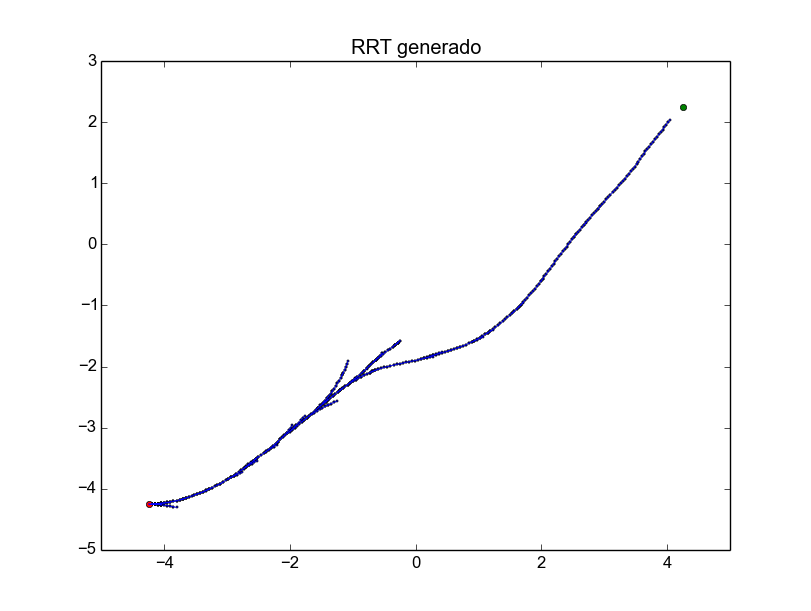
\includegraphics[scale=0.8]{imagenes/arbol_bias_alto.png}
        \caption{Árbol generado cuando se configura un bias alto}
    \end{center}
\end{figure}

\begin{figure}[ht]
    \begin{center}
        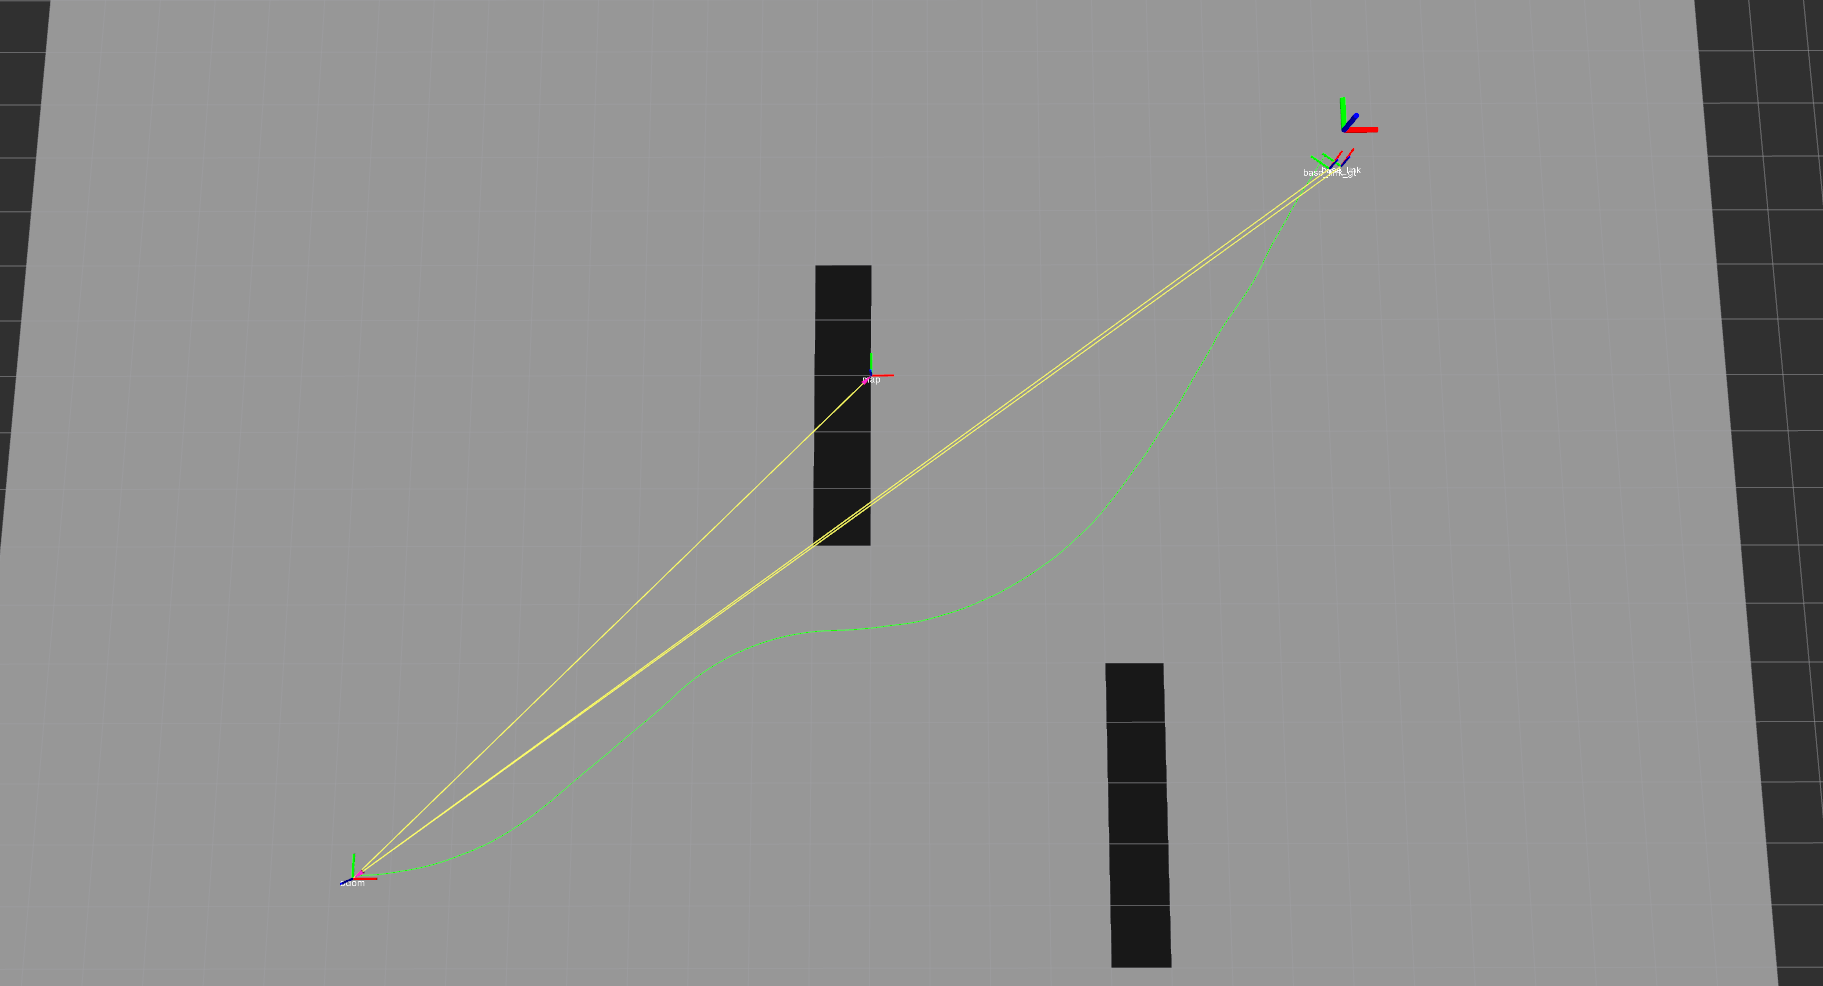
\includegraphics[scale=0.35]{imagenes/rviz_bias_alto.png}
        \caption{Camino calculado cuando se configura un bias alto}
    \end{center}
\end{figure}

\begin{figure}[ht]
    \begin{center}
        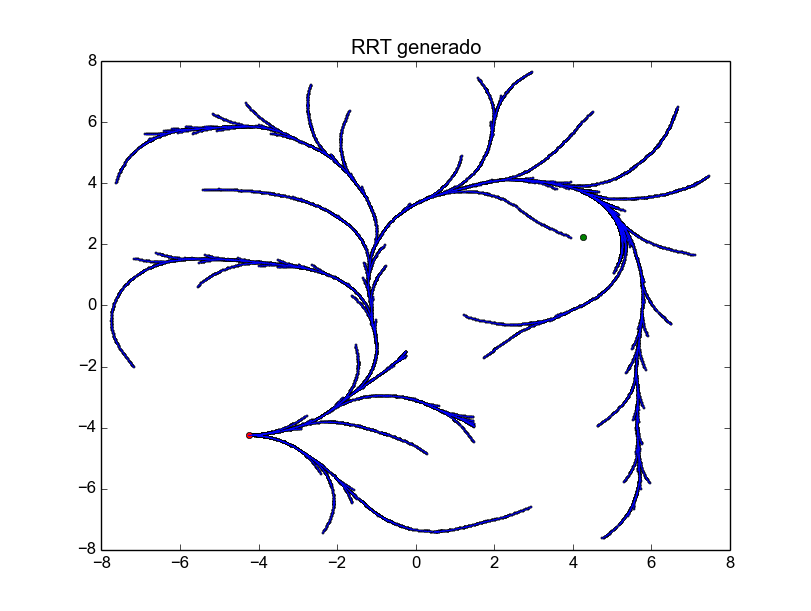
\includegraphics[scale=0.8]{imagenes/arbol_bias_bajo.png}
        \caption{Árbol generado cuando se configura un bias bajo}
    \end{center}
\end{figure}

\begin{figure}[ht]
    \begin{center}
        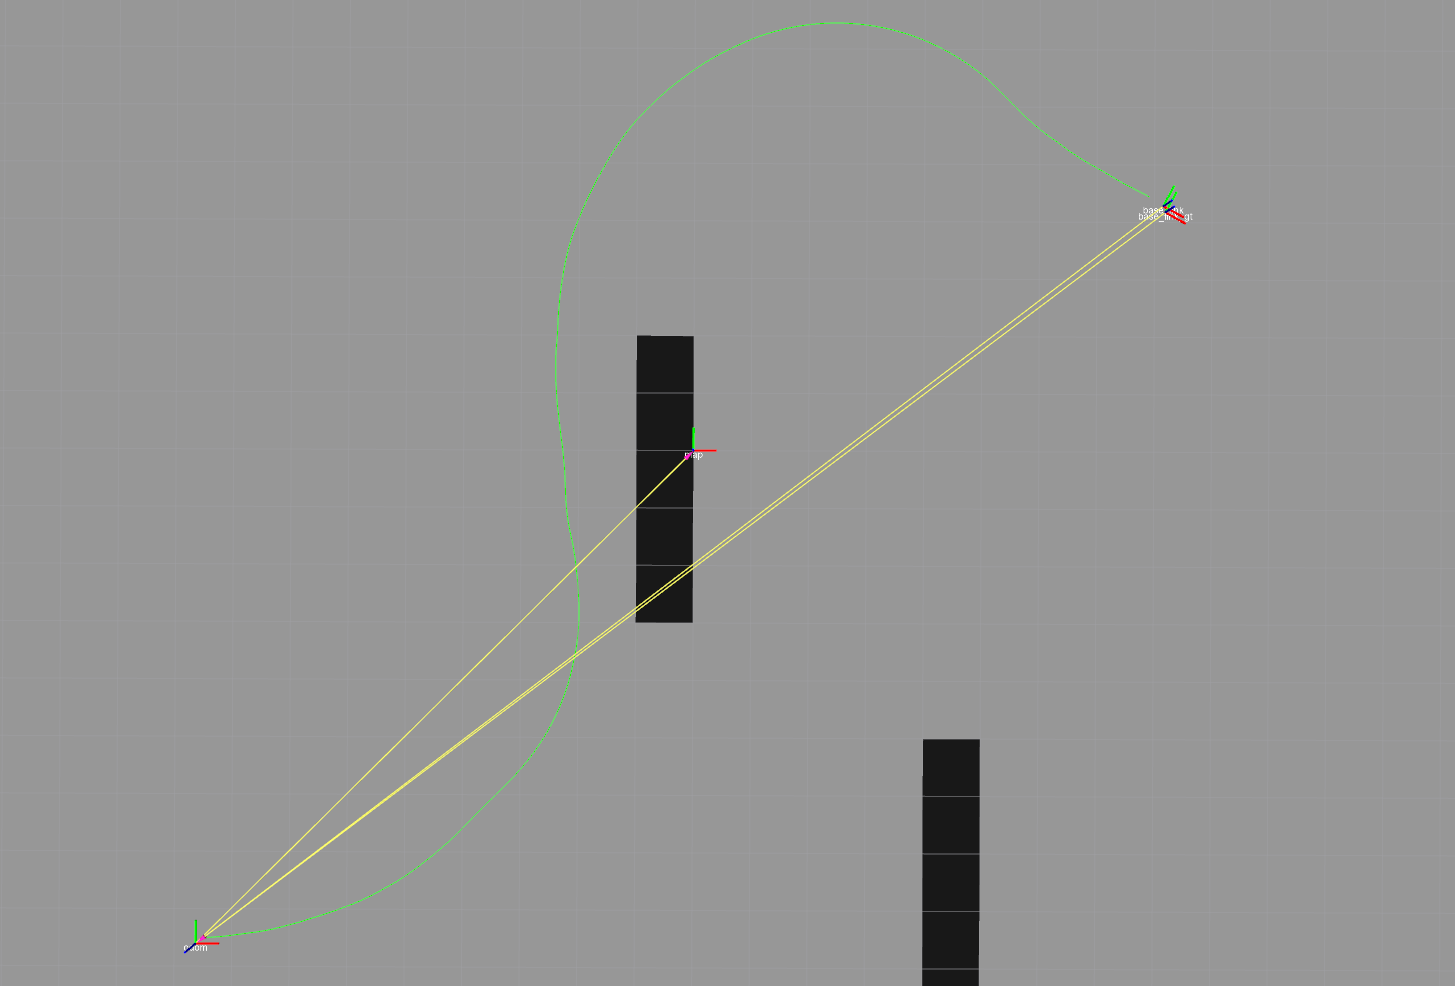
\includegraphics[scale=0.35]{imagenes/rviz_bias_bajo.png}
        \caption{Camino calculado cuando se configura un bias bajo}
    \end{center}
\end{figure}

\begin{figure}[ht]
    \begin{center}
        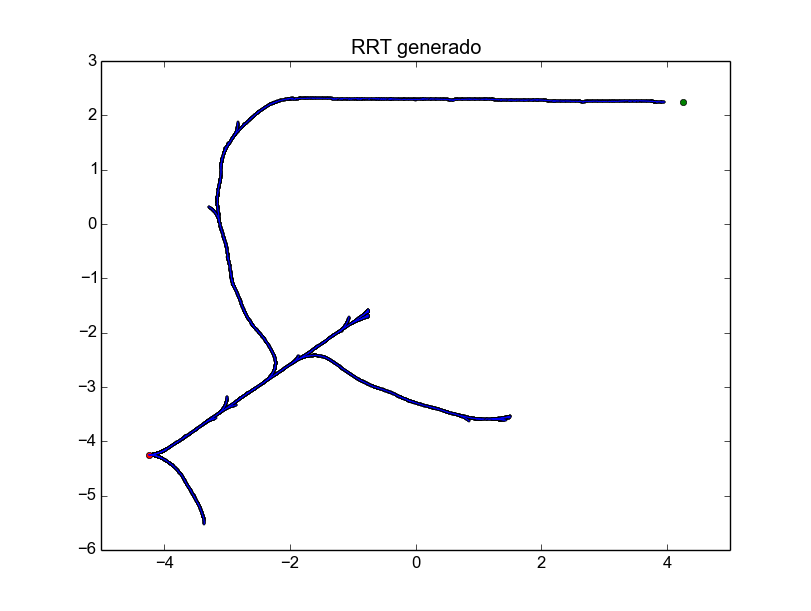
\includegraphics[scale=0.8]{imagenes/arbol_poco_demandante.png}
        \caption{Árbol generado cuando se configura con velocidades poco demandantes}
    \end{center}
\end{figure}

\begin{figure}[ht]
    \begin{center}
        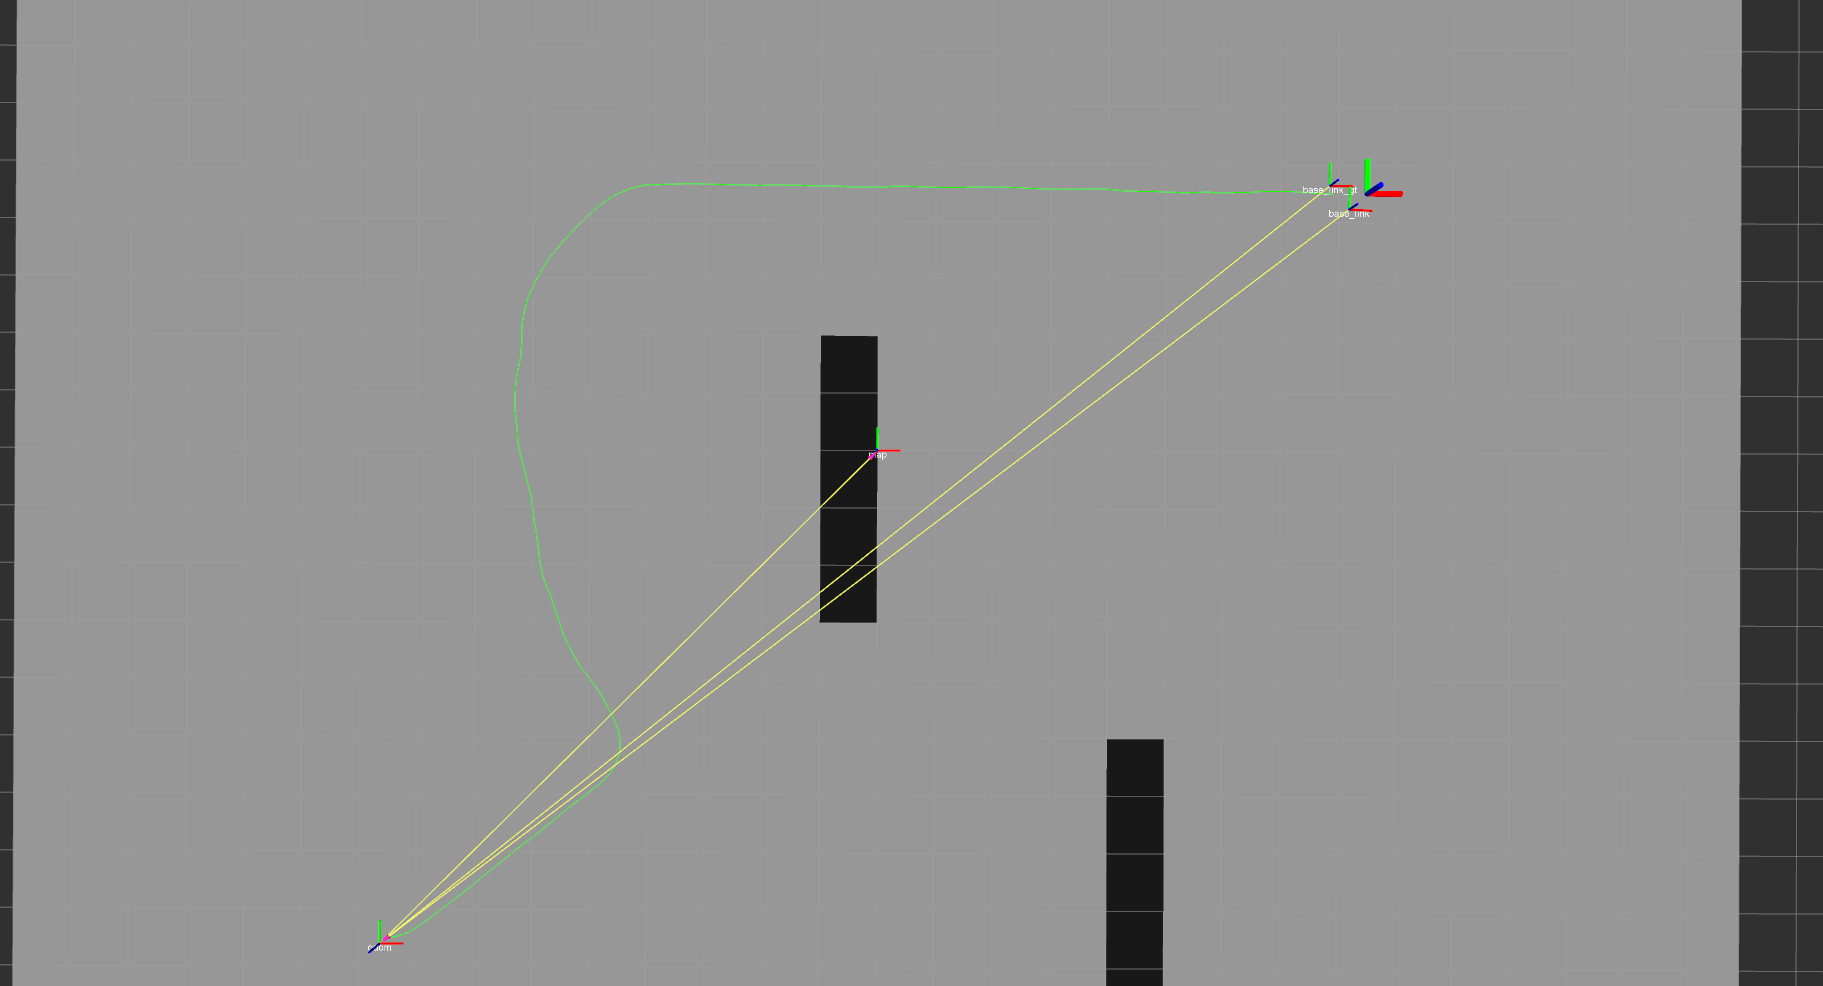
\includegraphics[scale=0.35]{imagenes/rviz_poco_demandante.png}
        \caption{Camino calculado cuando se configura con velocidades poco demandantes}
    \end{center}
\end{figure}

\begin{figure}[ht]
    \begin{center}
        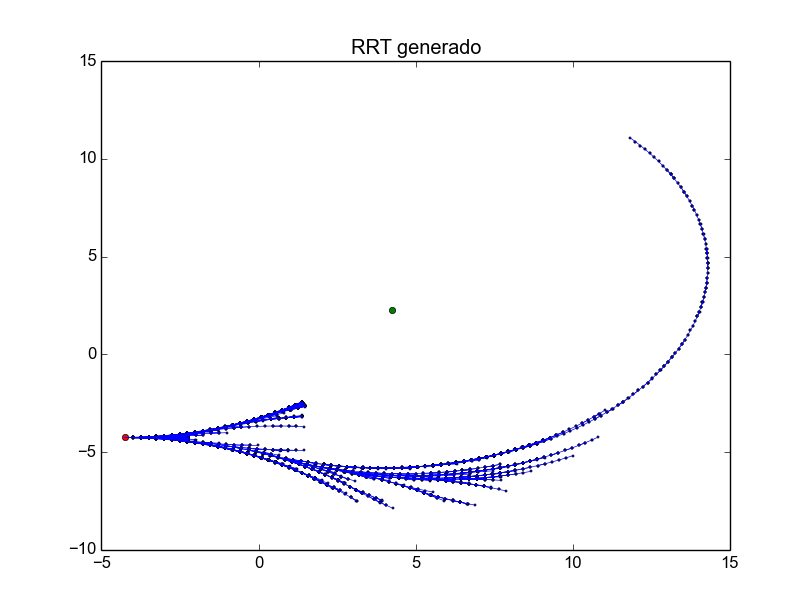
\includegraphics[scale=0.8]{imagenes/arbol_demandante.png}
        \caption{Árbol generado cuando se configura con velocidades demandantes}
    \end{center}
\end{figure}

\FloatBarrier
\subsection{¿Como se podría mejorar el algoritmo RRT de manera de ”guiarlo” de manera
más eficiente hacia el goal?. Contemplar el algoritmo A*.}

Podría calcularse un buen camino con A* para que al momento de generar los ``focos'' a donde el robot intentará dirigirse, este tenga en cuenta puntos del camino calculado. De esta forma el robot es guiado por la trayectoria de un camino bastante bueno.

Es importante que los puntos elegidos sean cercanos a los puntos explorados del árbol, ya que la ventaja de utilizar A* como guia es poder maniobrar mejor en senderos complicados. Si se toman puntos lejanos se pierde esa precisión.

\end{document}